
This dissertation begins with the coordinate system and kinematic variables used in collider experiments. They are followed by an overview of the relativistic heavy-ion collisions, and the \ac{sPHENIX} detector. The chapter concludes with the motivation and scope of this dissertation.


\section{Coordinate System and Kinematic Variables}
\label{app:additional_terms}


In this section, we introduce some of the technical terms and concepts commonly used in high-energy nuclear physics.


\subsection{Pseudorapidity (\texorpdfstring{$\eta$}{η})}

Pseudorapidity ($\eta$) is a spatial coordinate commonly used in collider physics to describe the angle of a particle relative to the beam axis. It is defined as:
\begin{equation}
\label{eq:pseudo_rap}
\eta = -\ln\left[\tan\left(\frac{\theta}{2}\right)\right]
\end{equation}


    
% figure for pseudo-rapidity
\begin{figure}[H]
  \centering
  \begin{minipage}{0.40\textwidth}
    \centering
    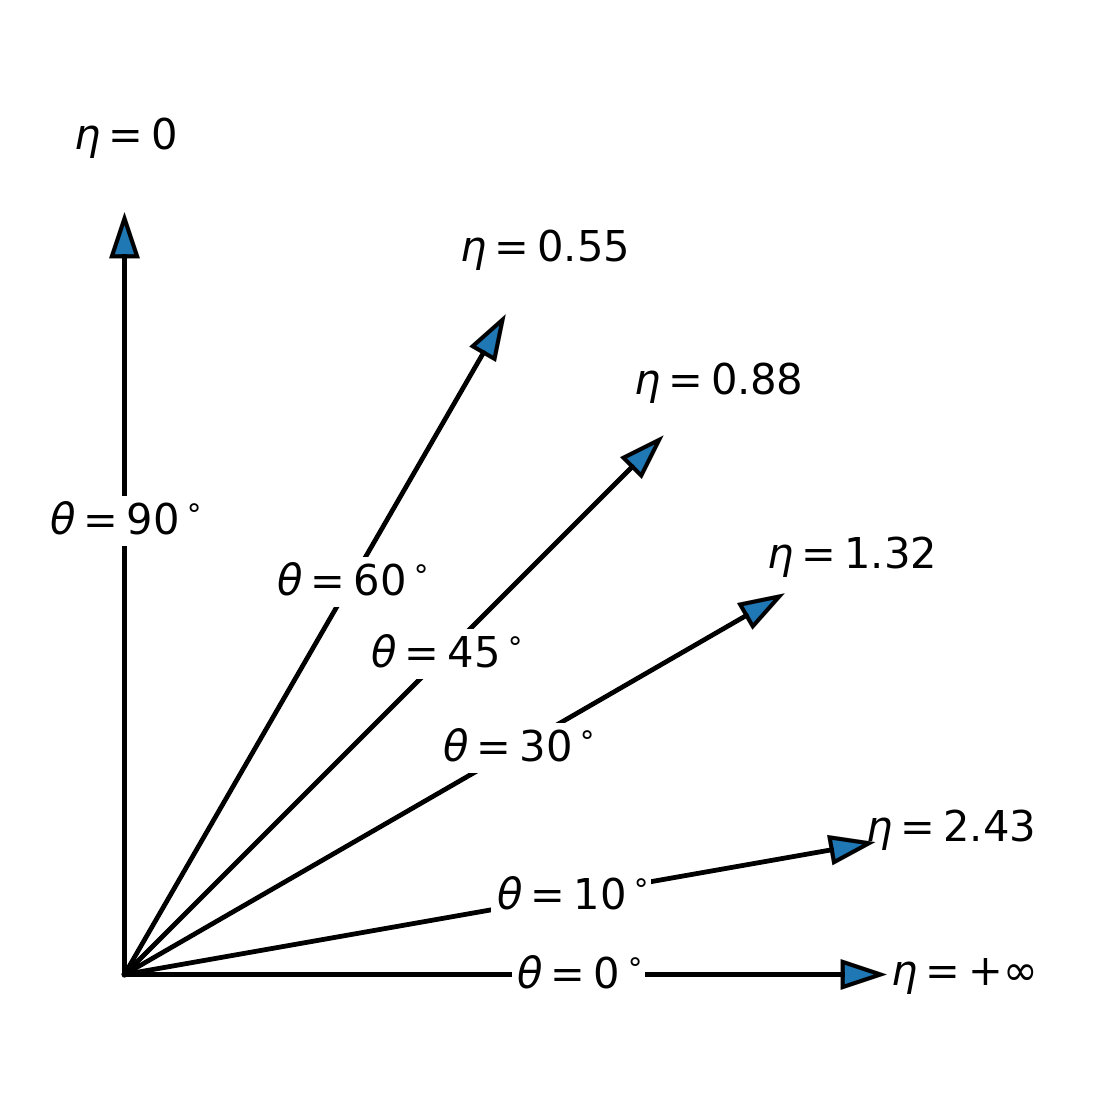
\includegraphics[width=\textwidth,
      alt={Diagram of arrows drawn from a common origin at polar angles of
           90, 60, 45, 30, 10 and 0 degrees, labeled with the corresponding
           pseudorapidity values eta = 0, 0.55, 0.88, 1.32, 2.43 and
           infinity.}]{Images/App/pseudorapidity_theta_diagram.png}
  \end{minipage}
  \hfill
  \begin{minipage}{0.50\textwidth}
    \centering
    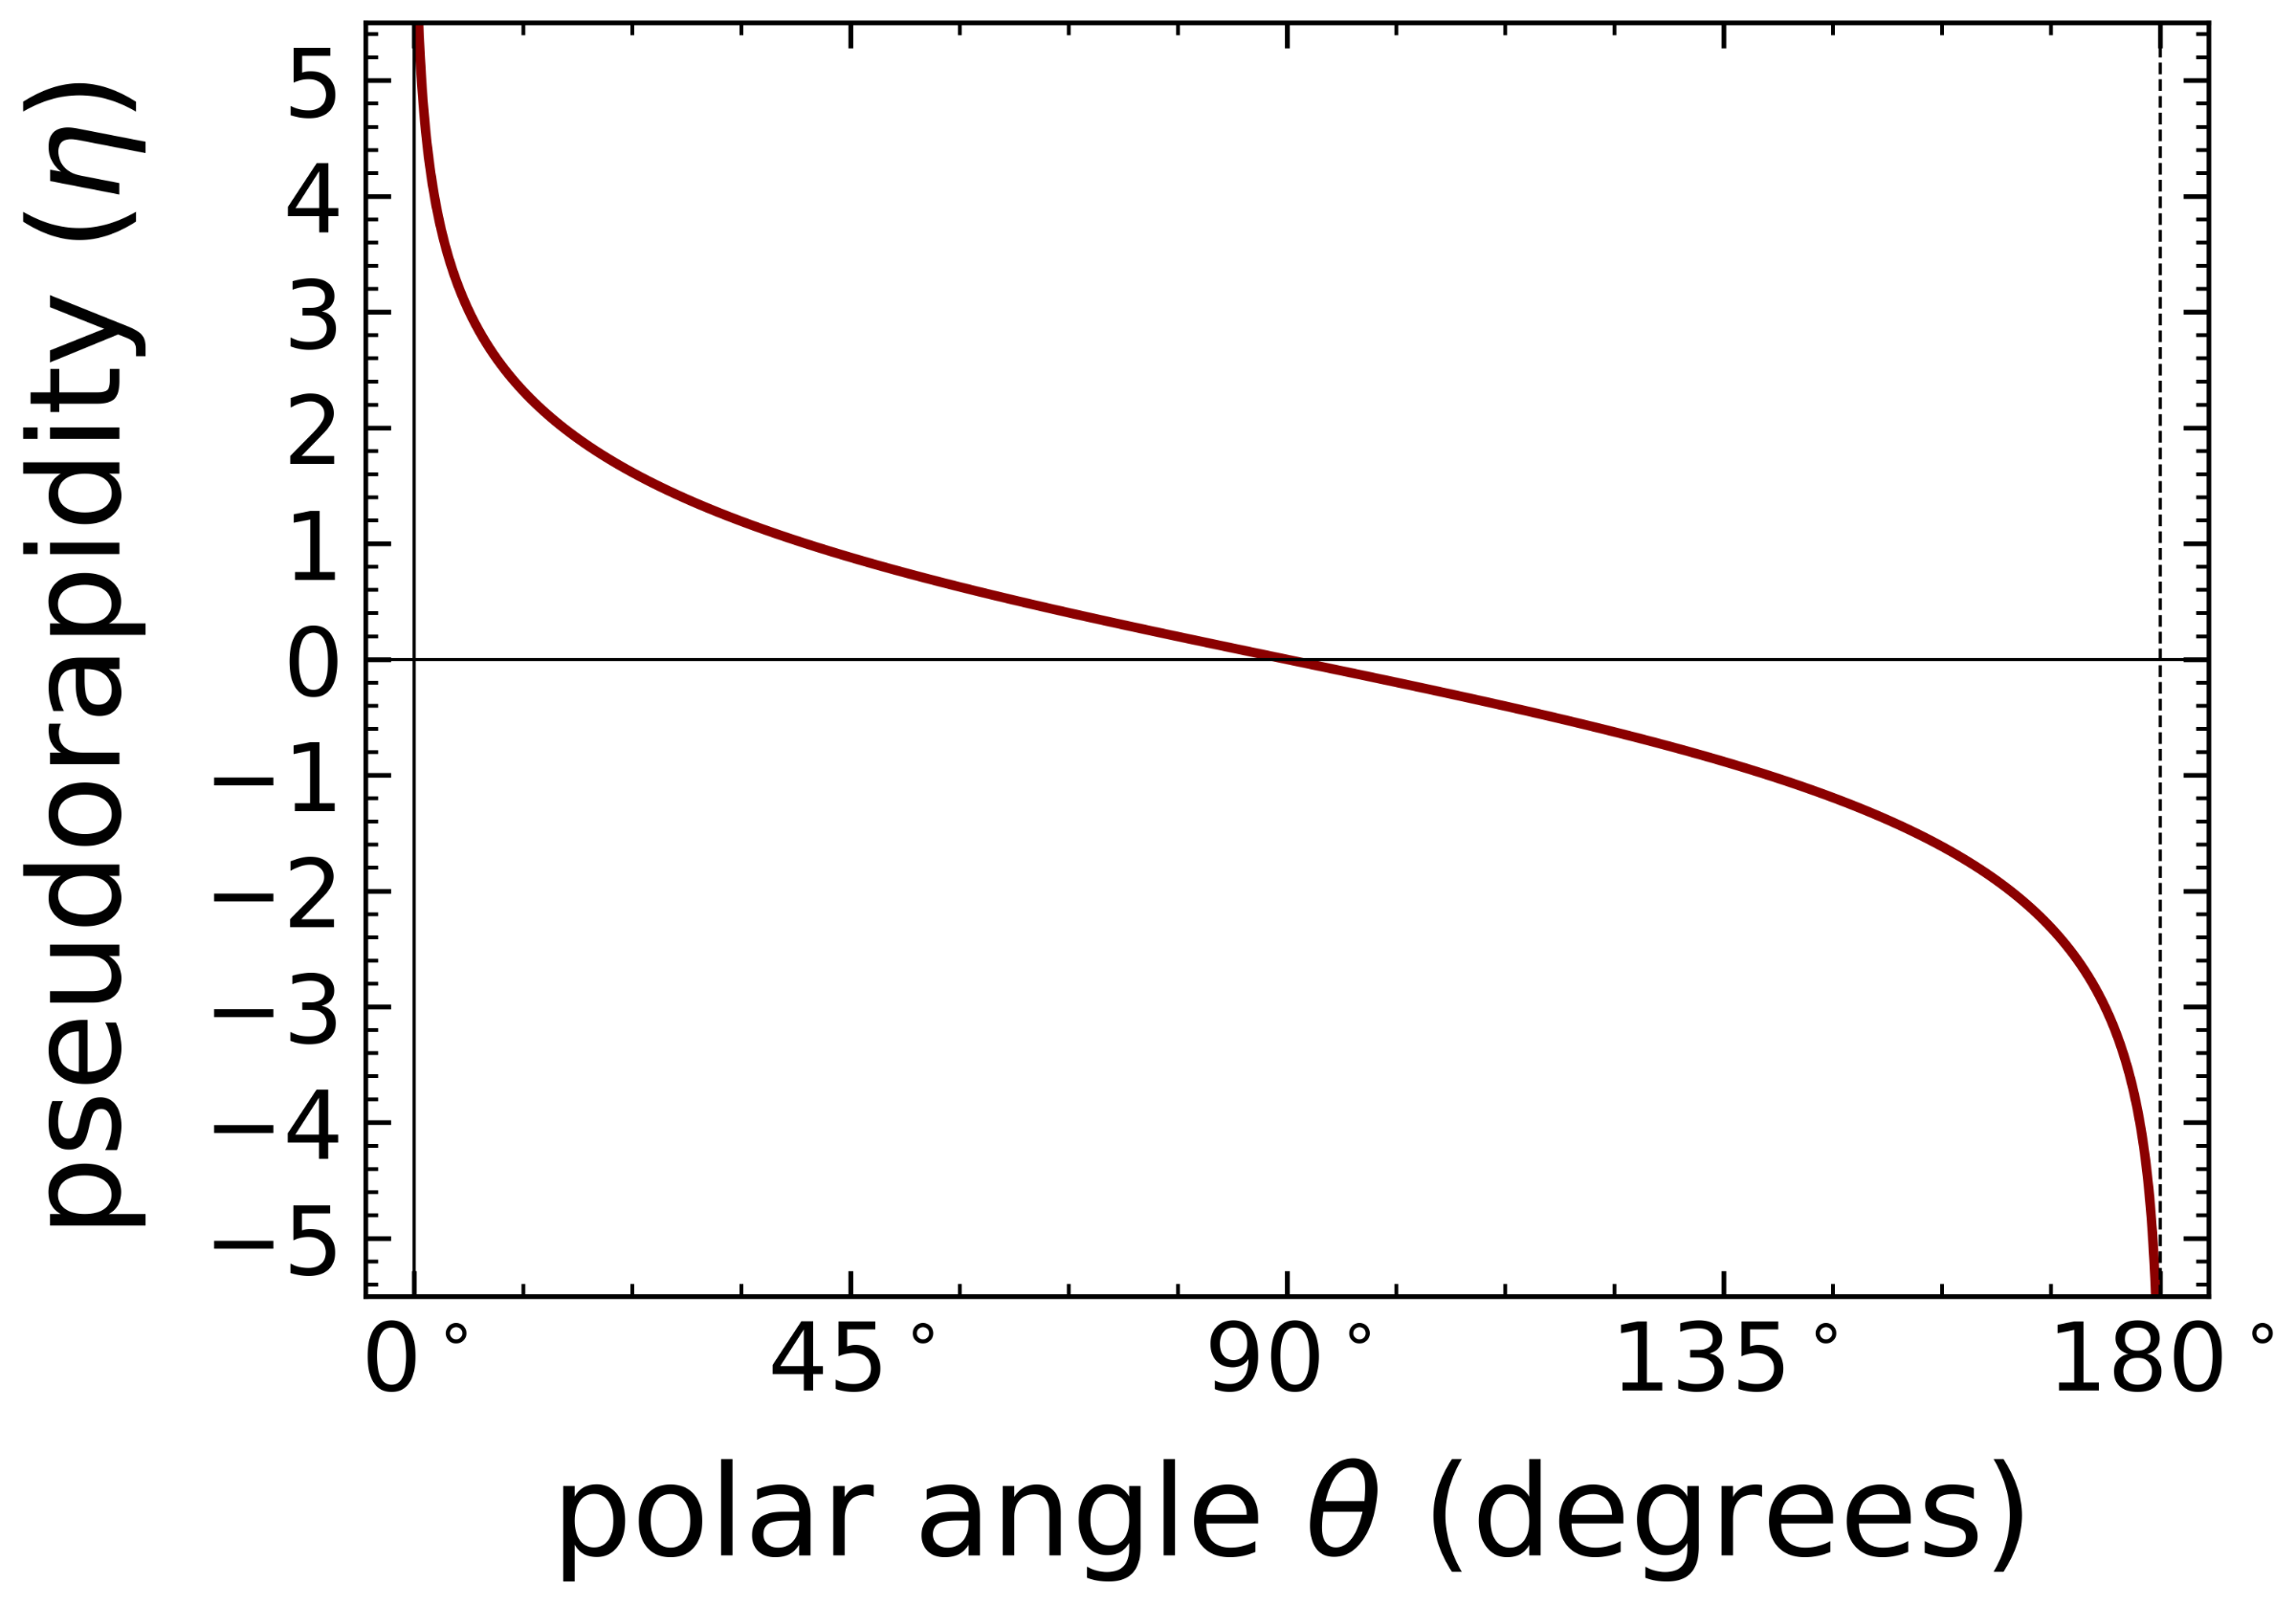
\includegraphics[width=\textwidth,
      alt={Plot of pseudorapidity eta versus polar angle theta from 0 to
           180 degrees. Eta falls from large positive values near 0 degrees,
           through zero at 90 degrees, to large negative values near
           180 degrees.}]{Images/App/eta_vs_theta.png}
  \end{minipage}
  \caption{Relationship between polar angle ($\theta$) and pseudorapidity ($\eta$): (a) geometric interpretation showing $\eta$ values for different polar angle $\theta$ ; (b) functional dependence of $\eta$ on $\theta$, illustrating its divergence as $\theta \to 0^\circ$ and $\theta \to 180^\circ$. Both images were created using Python.}
  \label{fig:pseudorapidity}
\end{figure}


From equation \ref{eq:pseudo_rap}, it is evident that pseudorapidity ($\eta$) is different mathematical form of the polar angle ($\theta$). Still, pseudorapidity is generally preferred over the polar angle as pseudorapidity ($\eta$) is closer to being a Lorentz invariant quantity. Pseudorapidity ($\eta$) acts as a proxy for rapidity ($y$) and achieves longitudinal boost invariance in the high-energy, massless limit. The relationship between pseudorapidity ($\eta$) and polar angle ($\theta$) is also reflected in the figure \ref{fig:pseudorapidity}.


